\documentclass{beamer}
\usepackage{tikz}
\graphicspath{ {./images/} }
\usepackage[usenames, dvipsnames]{color}
\usepackage[utf8]{inputenc}
\usepackage[english]{babel}


\begin{document}

\title{Smart Motor for Water Tanks}
\institute[Kerala Technological University] 
{
 \inst{}%
Department of Computer Science\\
College of Engineering, Trivandrum}
\author{Gokul K}
\date{February, 2019}

\begin{frame}

    \titlepage
\end{frame}

    \begin{frame}{Introduction}

        \begin{columns}
            \column{.5\textwidth}
                \includegraphics[height=.99\textwidth,width=.99\textwidth]{pic.png}
            \column{.5\textwidth}
                
               Most of the households in Kerala still depends on wells for water needs. Water from wells are pumped to overhead water tanks using motors. The traditional motors used can be improved using micro controllers to be water efficient and energy saving. We can also use sensors to measure and monitor the water level so as to prevent its wastage
                
        \end{columns}
    \end{frame}
    
     \begin{frame}{Need for a Smart Water Motor}
     \begin{itemize}
     
           \item Our water supply is finite, which means that we do not have an endless supply. Ninety - seven percent of all the water on the earth is salt water which is not suitable for drinking. Only three percent of all the water is fresh water, and only one percent is available for drinking water. The other two percent is locked in ice caps and glaciers.\break
           \item A lot of water is wasted during the operation of a water motor, since there is a delay in switching off the motor after the tank is filled.\break
           \item A smart water monitor helps households to plan and use water efficiently
    \end{itemize}
     \end{frame}
     \begin{frame}{Need for a Smart Water Motor}
     \centering
            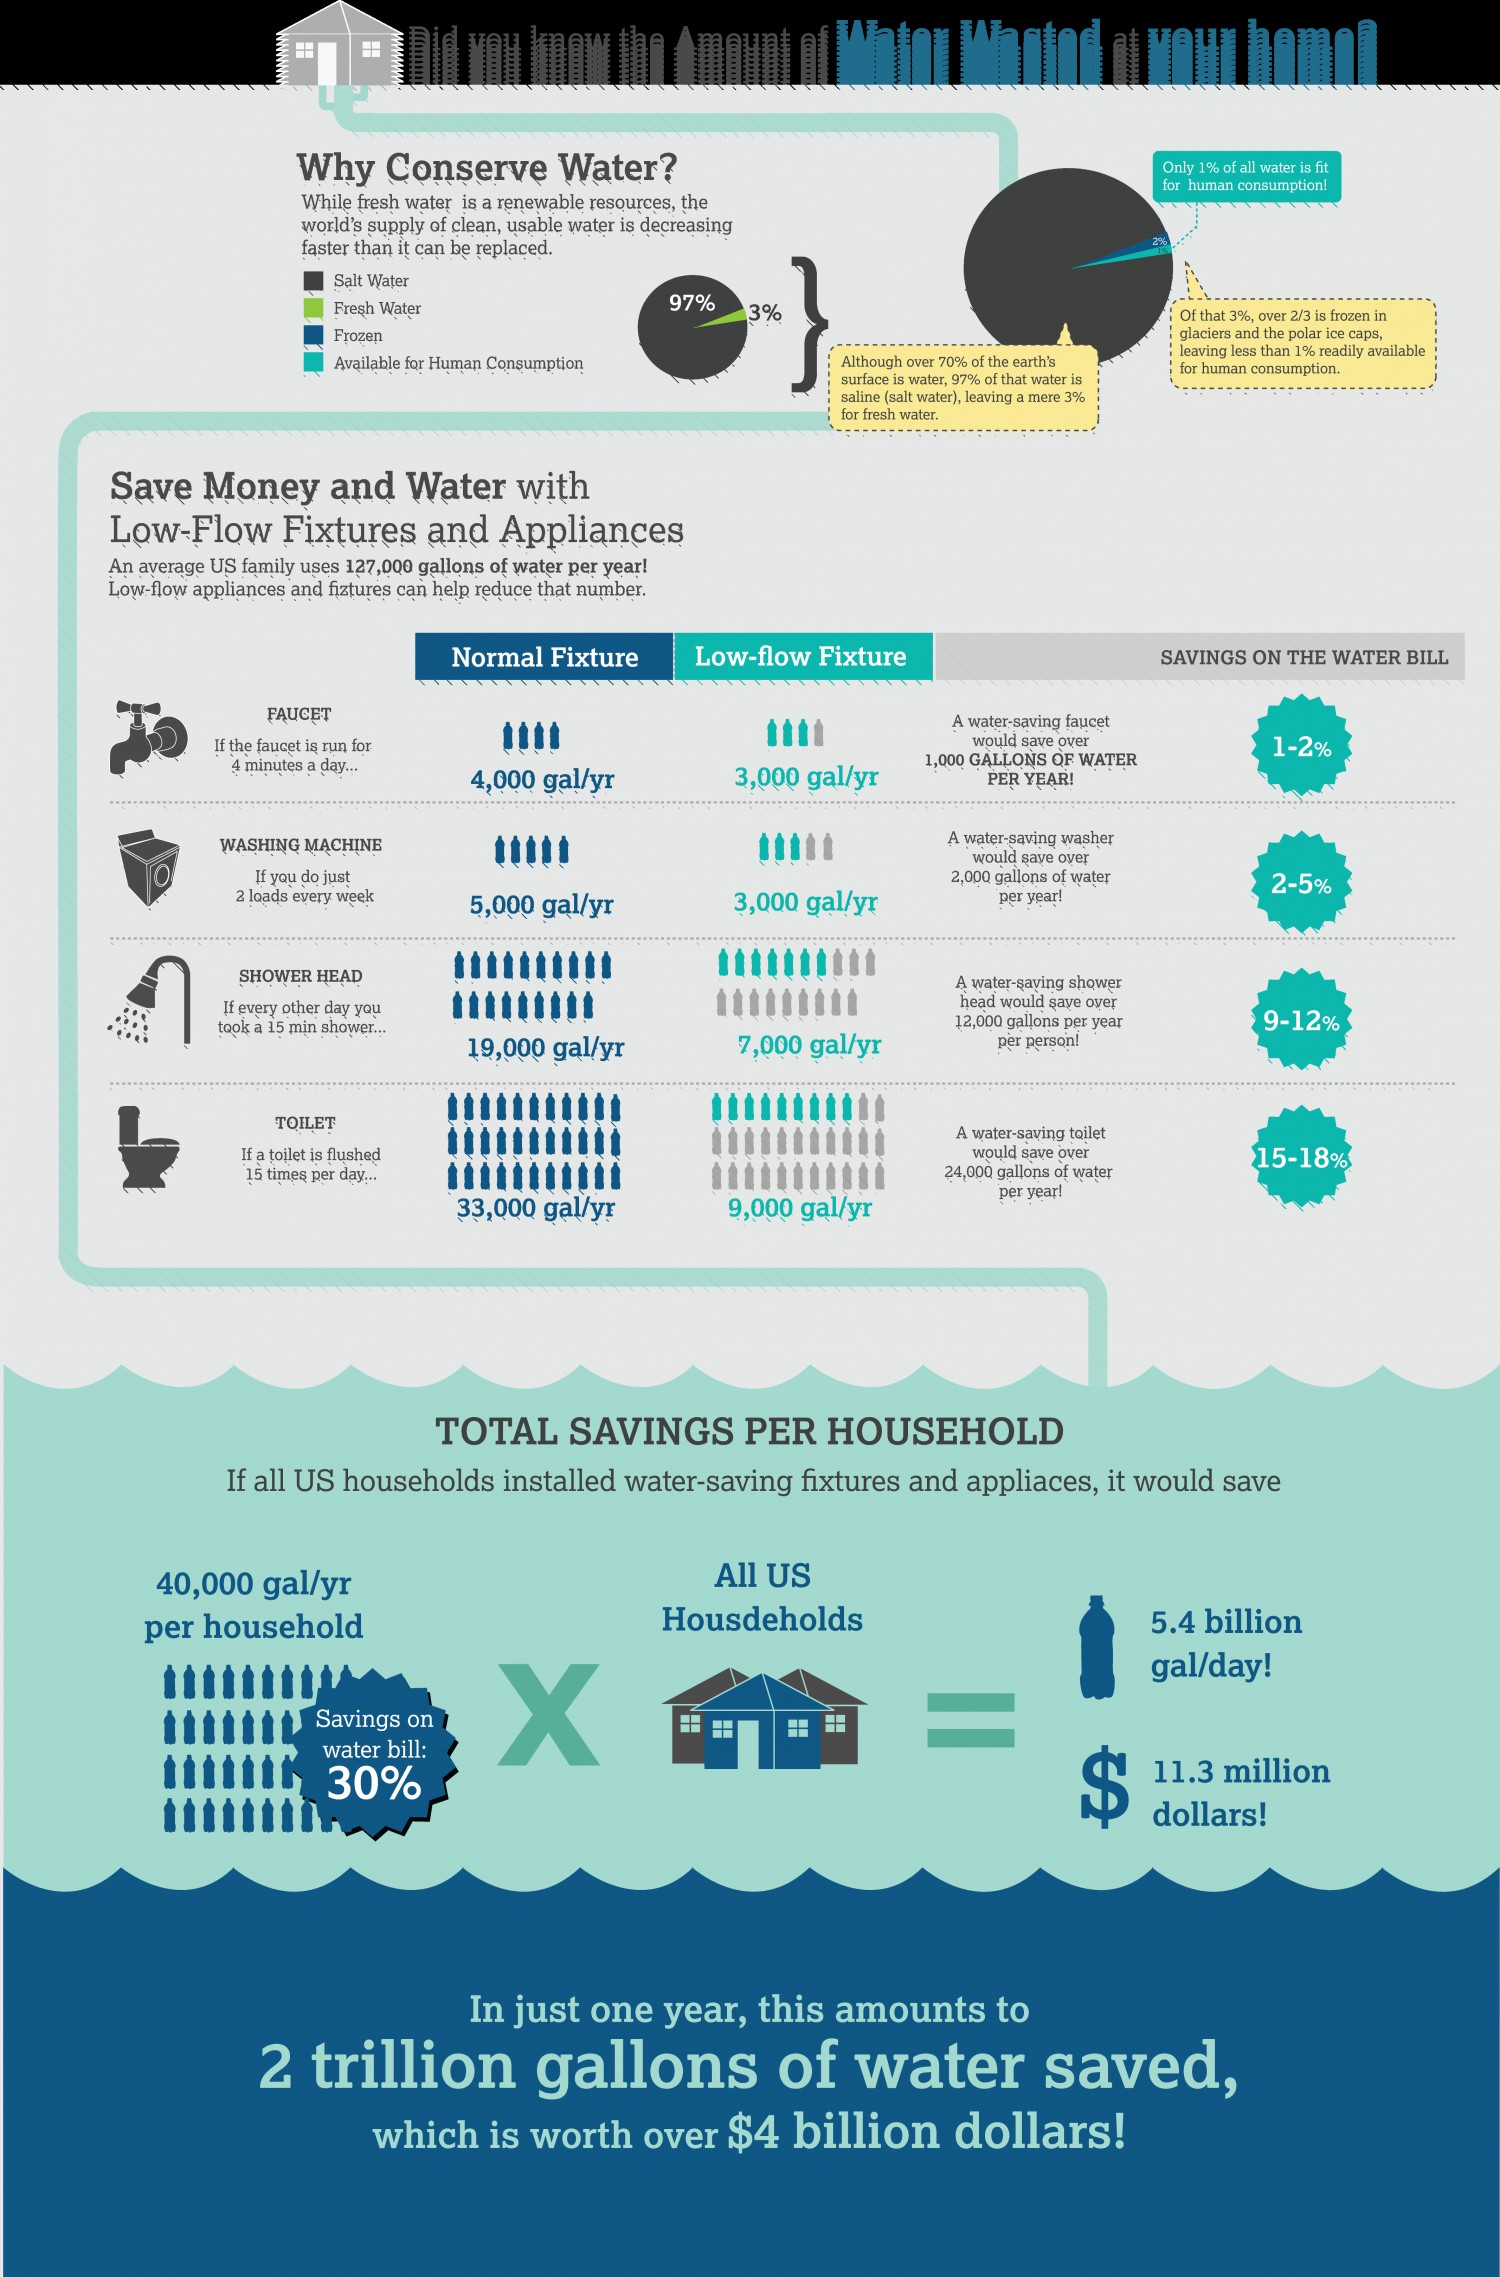
\includegraphics[width=.5\textwidth,height=.9\textheight]{img/water.png}
     \end{frame}
         
     
     \begin{frame}{Design Idea}\pause
        \begin{itemize}
            
            \item Water Monitor \break
            \begin{flushleft}
            An ultrasonic sensor is mounted on the water tank which will measure the water level in the tank. An ultrasonic (well above human hearing) pulse is transmitted from the unit and distance-to-target is determined by measuring the time required for the echo return. Output from the sensor is a variable-width pulse that corresponds to the distance to the target.\break
            \end{flushleft}
            \centering
            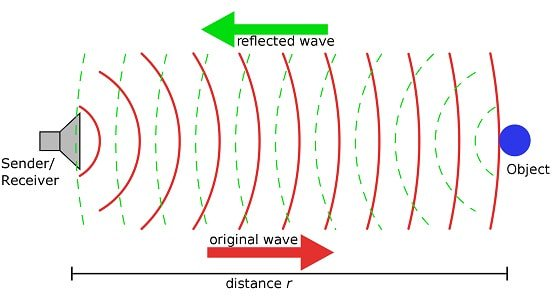
\includegraphics[width=.5\textwidth,height=.3\textheight]{img/ultrasonic.jpg}
            
         \end{itemize}
    \end{frame}
    \begin{frame}{Design Idea}
        \begin{itemize}
        \begin{flushleft}
        Using a micro processor, the water level is calculated and send to the motor system electrically.\break\break
        \end{flushleft}
        
        \item Water Motor \break
        \begin{flushleft}
        The Motor is equipped with a dashboard which displays the water level in the tank. The motor also provides an Auto option which automatically powers the motor when water level is low and turns off when it is full. Hence water loss can be prevented. Timely alerts will be provided when the water level is below a certain preset level. 
        \end{flushleft}
        \end{itemize}
     \end{frame}
       \begin{frame}{Conclusion}\pause
       \begin{itemize}
        \begin{flushleft}
           \item Water is vital for all known forms of life, even though it provides no calories or organic nutrients.\break
           \item Water wastage in households is a severe issue which contribute to the depletion of drinking water\break
           \item With right monitoring, we can plan our water usage to be sustainable\break
           \item This can be done using existing technology which is cheap and efficient\break
           \item A Smart Motor can also automate the turning on and off of a motor, which ensures the availability of water and reduces manual work
        \end{flushleft}
        \end{itemize}
    \end{frame}
    
    

\end{document}


